\section{Experiment Results}\label{sec_exp}

\newcommand{\mujocobaselinefigsize}{0.143}

We demonstrate the performance of our proposed algorithm (Sec. \ref{sec_exp_eval}) and ablate the different design choices (Sec. \ref{sec_exp_ablation}). Sec. \ref{sec_exp_init_sac} shows that the multi-task policy can serve as a good initialization, significantly speeding up training on unseen tasks. \autoref{sec_hyper_param} provides all hyper-parameters.


\subsection{Performance evaluation on unseen tasks}\label{sec_exp_eval}

% \fb{For fig 4 and 6, can you make the legend even bigger, maybe 1.5x. I still need to squint my eye to see them. I shorten the caption so you should have enough space.}

\begin{figure}[!t]
    \begin{minipage}{0.28\textwidth}
        \begin{figure}[H]
            \centering
            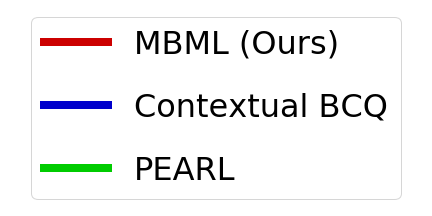
\includegraphics[width=\textwidth]{chapter_2/fig/legend_baseline.png}
            \caption{Results on unseen test tasks.
                x-axis is training epochs.
                y-axis is average episode returns.
                The shaded areas denote one std.
            }\label{fig:testing_performance}
        \end{figure}
    \end{minipage}
    \hfill
    \addtocounter{figure}{-1}
    \begin{minipage}{0.69\textwidth}

        \makebox[\textwidth]{

            \begin{subfigure}{\mujocobaselinefigsize\paperwidth}
                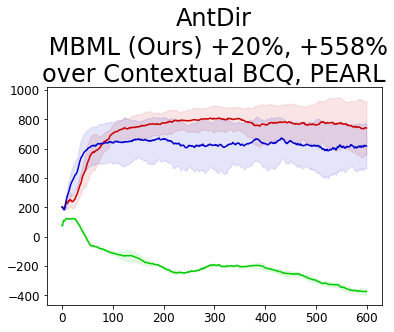
\includegraphics[width=\linewidth]{chapter_2/fig/wd-AntDir.png}
            \end{subfigure}

            \begin{subfigure}{\mujocobaselinefigsize\paperwidth}
                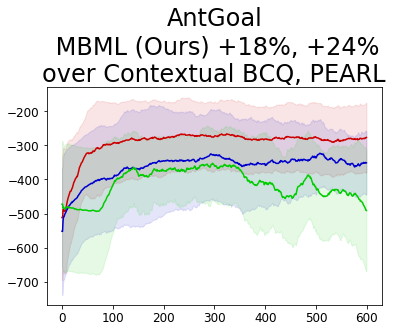
\includegraphics[width=\linewidth]{chapter_2/fig/wd-AntGoal.png}
            \end{subfigure}

            \begin{subfigure}{\mujocobaselinefigsize\paperwidth}
                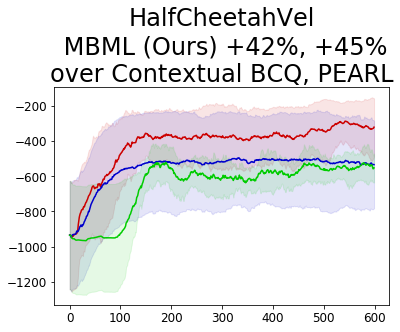
\includegraphics[width=\linewidth]{chapter_2/fig/wd-HalfCheetahVel.png}
            \end{subfigure}}

        \makebox[\textwidth]{
            \begin{subfigure}{\mujocobaselinefigsize\paperwidth}
                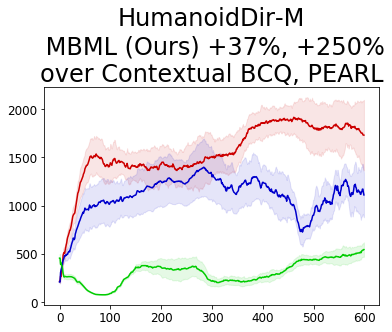
\includegraphics[width=\linewidth]{chapter_2/fig/wd-HumanoidDir-M.png}
            \end{subfigure}

            \begin{subfigure}{\mujocobaselinefigsize\paperwidth}
                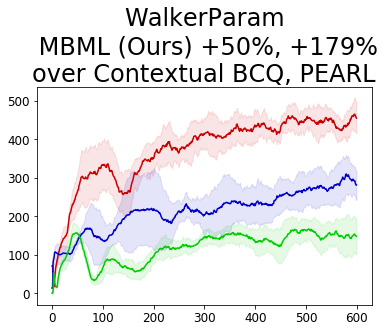
\includegraphics[width=\linewidth]{chapter_2/fig/wd-WalkerParam.png}
            \end{subfigure}

            \begin{subfigure}{\mujocobaselinefigsize\paperwidth}
                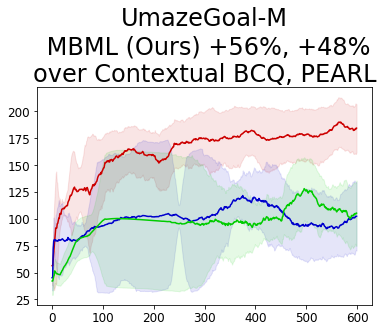
\includegraphics[width=\linewidth]{chapter_2/fig/wd-UmazeGoal-M.png}
            \end{subfigure}}

    \end{minipage}
\end{figure}

We evaluate in five challenging task distributions from MuJoCo \cite{todorov2012mujoco} and a modified task distribution UmazeGoal-M from D4RL \cite{fu2020d4rl}. In AntDir and HumanoidDir-M, a target direction defines a task. The agent maximizes returns by running with maximal speed in the target direction. In AntGoal and UmazeGoal-M, a task is defined by a goal location, to which the agent should navigate. In HalfCheetahVel, a task is defined as a constant velocity the agent should achieve. We also consider the WalkerParam environment where random physical parameters parameterize the agent, inducing different transition functions in each task. The state for each task distribution is the OpenAI gym state. We do not include the task-specific information, such as the goal location or the target velocity in the state. The target directions and goals are sampled from a $120^{\circ}$ circular arc. Details of these task distributions can be found in Appendix \ref{sec_env_detail}.

We argue that the version of HumanoidDir used in prior works does not represent a meaningful task distribution, where a single task policy can already achieve the optimal performance on unseen tasks. We thus modify the task distribution so that a policy has to infer the task identity to perform well, and denote it as HumanoidDir-M. More details of this task distribution can be found in \autoref{sec_humanoid}.

There are two natural baselines. The first is by modifying PEARL \cite{rakelly2019efficient} to train from the batch, instead of allowing PEARL to collect more transitions. We thus do not execute line $1-10$ in Algorithm 1 in the PEARL paper. On line 13, we sample the context and the RL batch uniformly from the batch. The second baseline is Contextual BCQ. We modify the networks in BCQ to accept the inferred task identity as input. We train the task inference module using the gradient of the value function loss. MBML and the baselines have the same network architecture. We are very much inspired by PEARL and BCQ. However, we do not expect PEARL to perform well in our setting because it does not explicitly handle the difficulties of learning from a batch without interactions. We also expect that our proposed algorithm will outperform Contextual BCQ thanks to more robust task inference.

We measure performance by the average returns over unseen tasks, sampled from the same task distribution. We do not count the first two episodes' returns \cite{rakelly2019efficient}. We obtain the batch for each training task by training Soft Actor Critic (SAC) \cite{haarnoja2018soft} with a fixed number of environment interactions. \autoref{sec_env_baseline} provide more details on the environment setups and training procedures of the baselines.

\begin{wrapfigure}{R}{0.259\textwidth}
    \vspace{-0.6em}
    \flushright
    \begin{subfigure}{0.155\paperwidth}
        % 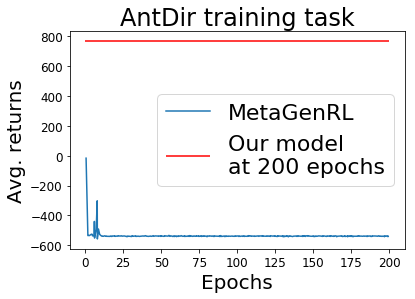
\includegraphics[width=\linewidth, right]{chapter_2/fig/metagenrl.png}
        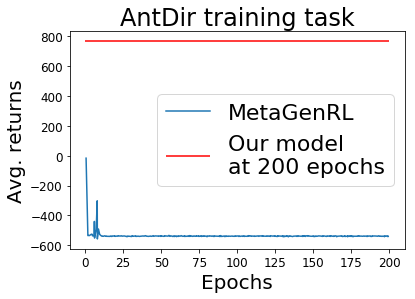
\includegraphics[width=\linewidth]{chapter_2/fig/metagenrl.png}
    \end{subfigure}
    \caption{MetaGenRL quickly diverges and does not recover.} %Results obtain from official MetaGenRL code.
    \label{fig:metagenrl}
    \vspace{0.05em}
\end{wrapfigure}

From Fig. \ref{fig:testing_performance}, MBML outperforms the baselines by a healthy margin in all task distributions. Even though PEARL does not explicitly handle the challenge of training from an offline batch, it is remarkably stable, only diverging in AntDir. Contextual BCQ is stable, but converges to a lower performance than MBML in all task distributions. An astude reader will notice the issue of overfitting, for example Contextual BCQ in HumanoidDir-M. Since our paper is not about determining early stopping conditions and to ensure fair comparisons among the different algorithms, we compute the performance comparisons using the best results achieved by each algorithm during training.

We also compare with MetaGenRL \cite{metagenrl}. Since it relies on DDPG \cite{ddpg} to estimate value functions, which diverges in Batch RL \cite{fujimoto2019off}, we do not expect it to perform well in our setting. Fig. \ref{fig:metagenrl} confirms this, where its performance quickly plummets and does not recover with more training.
Combining MetaGenRL and MBML is interesting since MetaGenRL generalizes to out-of-distribution tasks.


\subsection{Ablations}\label{sec_exp_ablation}

\begin{figure}[!t]
    \begin{minipage}{0.28\textwidth}
        \begin{figure}[H]
            \centering
            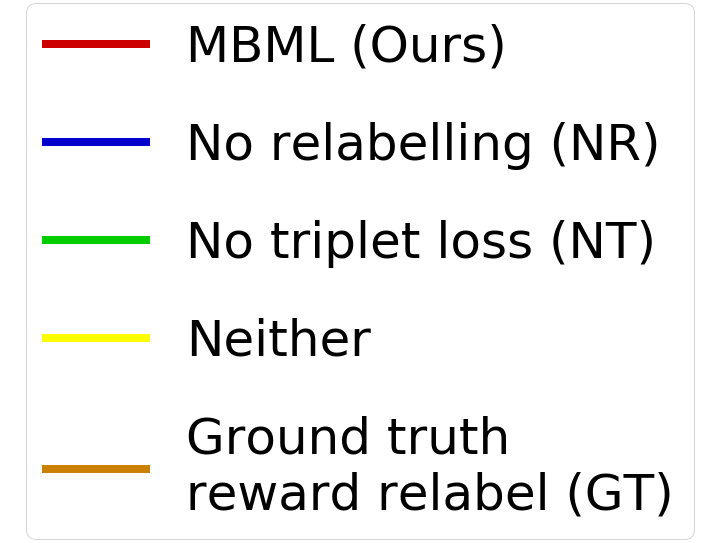
\includegraphics[width=\textwidth]{chapter_2/fig/legend_ablation.png}
            \caption{Ablation study.
                x-axis is training epochs.
                y-axis is average episode returns.
                The shaded areas denote one std.
            }\label{fig:ablation}
        \end{figure}
    \end{minipage}
    \hfill
    \addtocounter{figure}{-1}
    \begin{minipage}{0.70\textwidth}

        \makebox[\textwidth]{

            \begin{subfigure}{\mujocobaselinefigsize\paperwidth}
                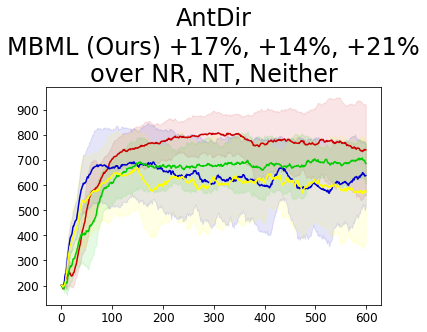
\includegraphics[width=\linewidth]{chapter_2/fig/wd-ablation-AntDir.png}
            \end{subfigure}

            \begin{subfigure}{\mujocobaselinefigsize\paperwidth}
                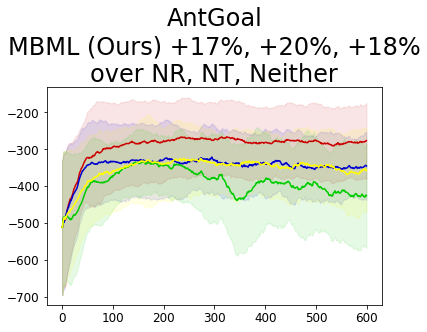
\includegraphics[width=\linewidth]{chapter_2/fig/wd-ablation-AntGoal.png}
            \end{subfigure}

            \begin{subfigure}{\mujocobaselinefigsize\paperwidth}
                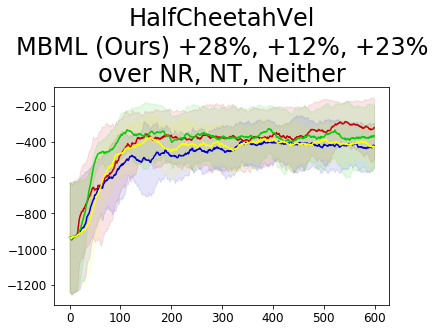
\includegraphics[width=\linewidth]{chapter_2/fig/wd-ablation-HalfCheetahVel.png}
            \end{subfigure}}

        \makebox[\textwidth]{
            \begin{subfigure}{\mujocobaselinefigsize\paperwidth}
                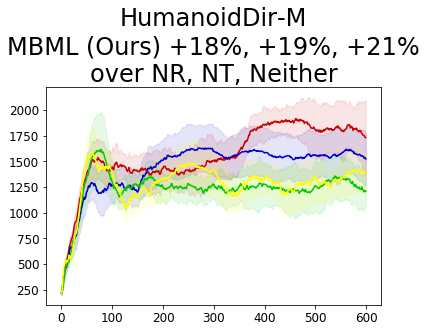
\includegraphics[width=\linewidth]{chapter_2/fig/wd-ablation-HumanoidDir-M.png}
            \end{subfigure}

            \begin{subfigure}{\mujocobaselinefigsize\paperwidth}
                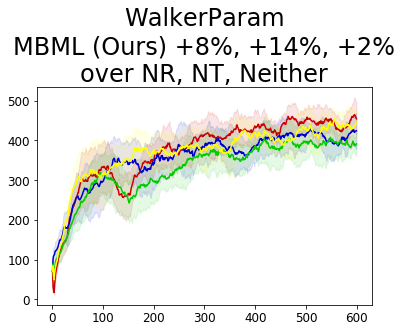
\includegraphics[width=\linewidth]{chapter_2/fig/wd-ablation-WalkerParam.png}
            \end{subfigure}

            \begin{subfigure}{\mujocobaselinefigsize\paperwidth}
                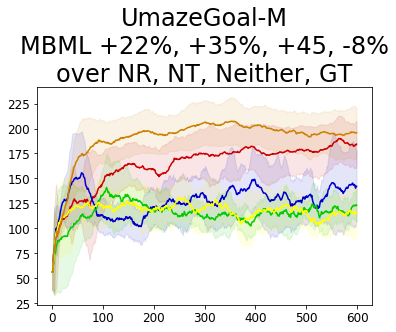
\includegraphics[width=\linewidth]{chapter_2/fig/wd-ablation-UmazeGoal-M.png}
            \end{subfigure}}

    \end{minipage}

\end{figure}

We emphasize that our contributions lie in the triplet loss design coupled with transitions relabelling. Below, we provide ablation studies to demonstrate that both are crucial to obtain superior performance.

\textbf{No relabelling.} To obtain  hard negative examples, we search over a mini-batch to find the hardest positive-anchor and negative-anchor pairs, a successful and strong baseline from metric learning \cite{hermans2017defense}. This requires sampling $N$ context sets $\{{\bf c}^n_i\}_{n=1}^N$ for each task $i$, where $n$ indexes the context sets sampled for each task.
Let $K$ be the number of training tasks, the triplet loss is:
\begin{equation}\label{eq_reform_triplet}
    \frac{1}{K} \sum_{i=1 }^{K} \bigg[\max_{n,n'=1,\ldots, N} \quad d \left(q_{\phi}({\bf c}^n_{i}\big), q_{\phi} ({\bf c}^{n'}_{i}) \right)
    -  \min_{\substack{n,n'=1,\ldots, N \\ j=1,\ldots,K, j \neq i}} \quad d \left(q_{\phi}({\bf c}^n_{i}\big), q_{\phi} ({\bf c}^{n'}_{j}) \right) + m\bigg]_{+}.
\end{equation}
The $max$ term
finds the positive-anchor pair
for task $i$
by considering every pair of context sets from task $i$ and selecting the pair with the largest divergence in the posterior over task identities. The $min$ term
finds the negative-anchor pair
for task $i$
by considering every possible pair between the context sets sampled for task $i$ and the context sets sampled for the other tasks. It then selects the pair with the lowest divergence in the posterior over task identities
as the negative-anchor pair.

\textbf{No triplet loss.} We train the task inference module using only gradient of the value function distillation loss (Eq. \ref{eq_loss_qi}).
To use the relabelled transitions, the module also takes as input the relabelled transitions during training.
More concretely, given the context set ${\bf c}_i$ from task $i$, we sample an equal number of relabelled transitions from the other tasks $\tilde{{\bf c}}_i \sim \cup_j {{\bf c}_{j \rightarrow{i} } }$. During training, the input to the task inference module is the union of the context set ${\bf c}_i$ and the sampled relabelled transitions $\tilde{{\bf c}}_i$. In the full model, we also perform similar modification to the input of the module during training.

\textbf{No transition relabelling and no triplet loss.} This method is a simple combination of a task inference module and the distillation process. We refer to this algorithm as \textbf{Neither} in the graphs.

Fig. \ref{fig:ablation} compares our full model and the ablated versions. Our full model obtains higher returns than most of the ablated versions. For WalkerParam, our full model does not exhibit improvement over  \textbf{Neither}. However, from Fig. \ref{fig:testing_performance}, our full model significantly outperforms the baselines. We thus conclude that, in WalkerParam, the improvement over the baselines comes from distillation.

\begin{wrapfigure}{R}{0.239\textwidth}
    \flushright
    \vspace{-0.5em}
    \begin{subfigure}{0.16\paperwidth}
        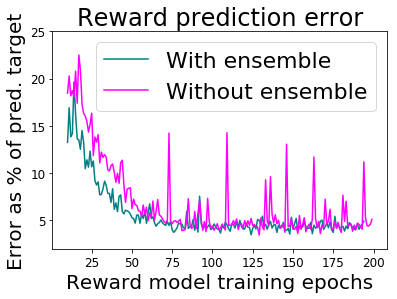
\includegraphics[width=\linewidth]{chapter_2/fig/reward_pred_error.png}
    \end{subfigure}
    \caption{Error on unseen task.}\label{fig:reward_error}
    \vspace{-0.2em}
\end{wrapfigure}

Comparing to the \textbf{No triplet loss} ablation, transition relabelling leads to more efficient computation of the triplet loss. Without the relabelled transitions, computing Eq. \ref{eq_reform_triplet} requires $O(K^2 N^2)$. Our loss in Eq. \ref{eq_triplet_all_task} only requires $O(K^2)$. We also need to relabel the transitions only once before training the multi-task policy. It is also trivial to parallelize across tasks.

We also study reward estimation accuracy. Fig. \ref{fig:reward_error} shows that our reward model achieves low error on state-action pairs from another task, both with and without an ensemble. We also compare MBML against an ablated version that uses the ground truth reward function for relabelling on UmazeGoal-M. The model trained using the ground truth reward function only performs slightly better than the model trained using the learned reward function. We include in \autoref{sec_ablation} experiments on margin sensitivity analysis and the benefit of the reward ensemble.

\subsection{Using the multi-task policy to enable faster convergence when training on unseen tasks}\label{sec_exp_init_sac}

While the multi-task policy generalize to unseen tasks, its performance is not optimal. If we allow further training,
initializing networks with our multi-task policy significantly speeds up convergence to the optimal performance.

The initialization process is as followed. Given a new task, we use the multi-task policy to collect 10K transitions.
We then train a new policy to imitate the actions taken by maximizing their log likelihood. As commonly done, the new policy outputs the mean and variance of a diagonal Gaussian distribution. The new policy does not take a task identity as input. The task inference module infers a task identity {\bf z} from the 10K transitions. Fixing {\bf z} as input, the distilled value function $Q_D$ initializes the new value function. Given the new policy and the initialized value function,
we train them with SAC by collecting more data.
To stabilize training, we perform target policy smoothing \cite{TD3} and double-Q learning \cite{van2016deep} by training two identically initialized value functions with different mini-batches (pseudo-codes and more motivations in Appendix \ref{sec_sac_our_methods}).

Fig. \ref{fig:SAC_init} compares the performance of the policies initialized with our multi-task policy to randomly initialized policies.
Initializing the policies with the MBML policy significantly increases convergence speed in all five task distributions, demonstrating our method's robustness.
Even in the complex HumanoidDir-M task distribution, our method significantly speeds up the convergence, requiring only 85K environment interactions, while the randomly initialized policies require 350K, representing a $76\%$ improvement in sample efficiency.
Similar conclusions hold when comparing against randomly initialized SAC where the two value functions are trained using different mini-batches (Appendix \ref{sec_init_counterpart}).
We also note that our initialization method does not require extensive hyper-parameter tuning.

% \fb{Your changes in the appendix lgtm. You can remove the blue color from them.}

\begin{figure*}[t]
    \centering
    \makebox[\textwidth]{
        \begin{subfigure}{0.125\paperwidth}
            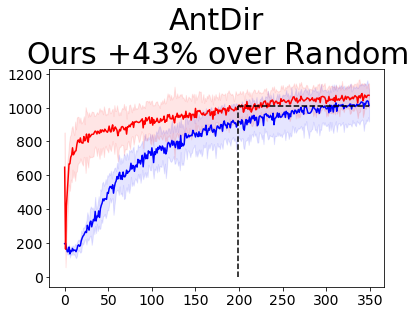
\includegraphics[width=\linewidth]{chapter_2/fig/init-sac-vs-train-AntDir.png}
        \end{subfigure}

        \begin{subfigure}{0.125\paperwidth}
            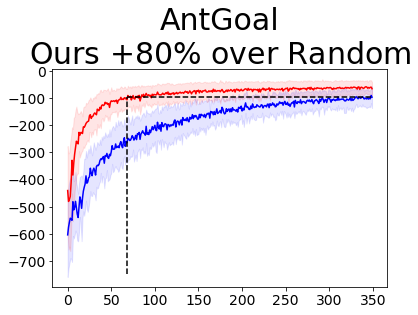
\includegraphics[width=\linewidth]{chapter_2/fig/init-sac-vs-train-AntGoal.png}
        \end{subfigure}

        \begin{subfigure}{0.125\paperwidth}
            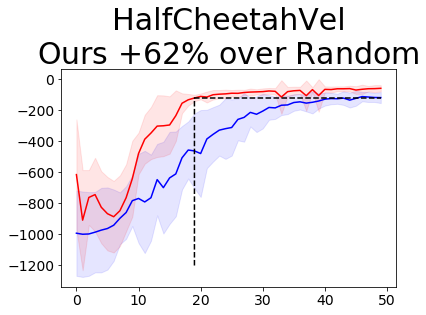
\includegraphics[width=\linewidth]{chapter_2/fig/init-sac-vs-train-HalfCheetahVel.png}
        \end{subfigure}

        \begin{subfigure}{0.125\paperwidth}
            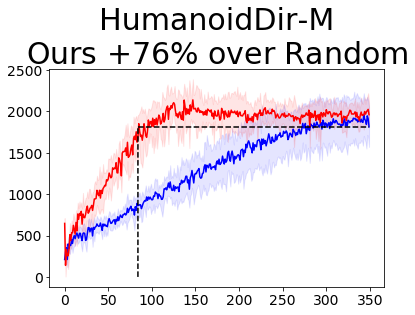
\includegraphics[width=\linewidth]{chapter_2/fig/init-sac-vs-train-HumanoidDir-M.png}
        \end{subfigure}

        \begin{subfigure}{0.125\paperwidth}
            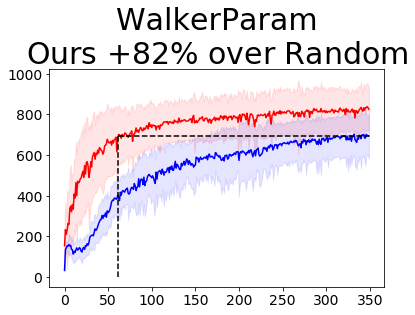
\includegraphics[width=\linewidth]{chapter_2/fig/init-sac-vs-train-WalkerParam.png}
        \end{subfigure}}
    \small{\color{red}--- }: SAC initialized by our multi-task policy (Ours) \qquad  {\color{blue}--- }: Randomly initialized SAC (Random)
    \caption{Initialization results.
        x-axis is number of interactions in thousands.
        y-axis is the average episode returns over unseen tasks.
        The shaded areas denote one std. }
    \label{fig:SAC_init}
\end{figure*}
